% Copyright (c) 2026 by C. Klukas.
% Licensed under the MIT License. See LICENSE for details.

\documentclass[11pt,a4paper]{article}

\usepackage[T1]{fontenc}
\usepackage[utf8]{inputenc}
\usepackage{libertinus}
\usepackage{microtype}
\usepackage[a4paper,margin=28mm,headheight=22pt]{geometry}
\usepackage{booktabs}
\usepackage{caption}
\usepackage{enumitem}
\usepackage{fancyhdr}
\usepackage{float}
\usepackage{graphicx}
\usepackage{needspace}
\usepackage{xcolor}
\usepackage{tikz}
\usepackage{listings}
\usepackage{titlesec}
\usepackage{hyperref}
\usepackage{url}
\usetikzlibrary{arrows.meta,fit,positioning}

\definecolor{pagletsBlue}{HTML}{1F5A85}
\definecolor{pagletsInk}{HTML}{1F2933}
\definecolor{pagletsMuted}{HTML}{5F6B76}
\definecolor{pagletsRule}{HTML}{B8C7D3}
\definecolor{pagletsCode}{HTML}{F6F8FA}

\hypersetup{
  colorlinks=true,
  linkcolor=pagletsBlue,
  citecolor=pagletsBlue,
  urlcolor=pagletsBlue,
  pdftitle={Paglets: Explicit-State Mobile Agents for Python Host Meshes},
  pdfauthor={Christian Klukas}
}

\AtBeginDocument{\color{pagletsInk}}

\titleformat{\section}
  {\Large\bfseries\color{pagletsBlue}}
  {\thesection}{0.75em}{}
\titleformat{\subsection}
  {\large\bfseries\color{pagletsBlue!85!black}}
  {\thesubsection}{0.65em}{}
\titlespacing*{\section}{0pt}{2.6ex plus 0.6ex minus 0.2ex}{1.2ex}
\titlespacing*{\subsection}{0pt}{2.0ex plus 0.4ex minus 0.2ex}{0.8ex}

\captionsetup{
  font=small,
  labelfont={bf,color=pagletsBlue},
  labelsep=period
}

\setlist{itemsep=0.25em,topsep=0.45em}
\renewcommand{\arraystretch}{1.05}

\pagestyle{fancy}
\fancyhf{}
\fancyhead[L]{\small\textsc{Paglets}}
\fancyhead[R]{\small\thepage}
\renewcommand{\headrulewidth}{0.25pt}
\renewcommand{\headrule}{\hbox to\headwidth{\color{pagletsRule}\leaders\hrule height \headrulewidth\hfill}}
\renewcommand{\footrulewidth}{0pt}

\renewenvironment{abstract}
  {\begin{center}\begin{minipage}{0.92\linewidth}\small\noindent\textbf{Abstract.}\quad}
  {\end{minipage}\end{center}\vspace{0.6em}}

\lstdefinestyle{paglets-python}{
  language=Python,
  basicstyle=\small\ttfamily,
  keywordstyle=\color{pagletsBlue},
  commentstyle=\color{pagletsMuted},
  stringstyle=\color{green!35!black},
  showstringspaces=false,
  breaklines=true,
  backgroundcolor=\color{pagletsCode},
  frame=single,
  framerule=0.3pt,
  rulecolor=\color{pagletsRule},
  columns=fullflexible
}

\tikzset{
  pagletsLayer/.style={
    draw=pagletsRule,
    fill=pagletsCode,
    rounded corners=2pt,
    line width=0.45pt,
    align=center,
    inner xsep=8pt,
    inner ysep=7pt,
    text width=0.55\linewidth
  },
  pagletsSide/.style={
    draw=pagletsRule,
    fill=white,
    rounded corners=2pt,
    line width=0.45pt,
    align=center,
    inner xsep=6pt,
    inner ysep=6pt,
    text width=0.15\linewidth
  },
  pagletsArrow/.style={
    -{Latex[length=2.1mm,width=1.6mm]},
    draw=pagletsBlue,
    line width=0.55pt
  },
  pagletsMeshArrow/.style={
    {Latex[length=2.1mm,width=1.6mm]}-{Latex[length=2.1mm,width=1.6mm]},
    draw=pagletsBlue,
    line width=0.55pt
  }
}

\begin{document}
\thispagestyle{plain}
\begin{center}
{\LARGE\bfseries\color{pagletsBlue}Paglets: Explicit-State Mobile Agents for Python Host Meshes\par}
\vspace{0.65em}
{\large Christian Klukas\footnote{\href{https://orcid.org/0000-0001-7956-0294}{ORCID: 0000-0001-7956-0294}}\par}
\vspace{0.25em}
{\small\color{pagletsMuted}June 23, 2026\par}
\vspace{0.9em}
{\color{pagletsRule}\rule{\linewidth}{0.7pt}}
\end{center}
\vspace{0.8em}

\begin{abstract}
Mobile agents offered a direct programming model for computations that move
between networked hosts, carrying behavior and state closer to the resources
they need. IBM's Java Aglets system made this idea concrete with a mobile-agent
API, proxies, message passing, dispatch, retraction, activation, and
deactivation. Paglets revisits the same family of ideas for modern Python, but
deliberately narrows the mobility model: code is not uploaded at movement time,
Python stacks and live resources do not migrate, and every mobile object carries
explicit dataclass state that can be serialized, inspected, persisted, and
moved between trusted hosts. This paper introduces the Paglets
runtime, explains how it relates to Aglets, and outlines practical use cases
for infrastructure inspection, data-local analytics, distributed examples, and
stateful agent workflows. A small two-host evaluation illustrates movement
latency, payload transfer speed, and host-local benchmark behavior on a mixed
macOS and Windows mesh.
\end{abstract}

\noindent\textbf{Keywords:} mobile agents; Python; Aglets; distributed systems;
dataclass state; process isolation; trusted meshes

\section{Introduction}

Most distributed applications are written as stationary services. A client sends
requests to a server, the server performs an operation, and state usually stays
behind an API boundary. This model is reliable and familiar, but it is not the
only useful way to think about distributed computation. In several workflows the
unit of work is naturally stateful, long-running, and location-aware: it should
visit hosts, inspect local context, talk to resident services, keep progress,
and return with a compact result. The mobile-agent literature explored this
model in the 1990s and asked when it was better to move a computation than to
move all data and control traffic through a central process
\cite{harrison1995mobileAgents,lange1997aglets}.

Paglets is a compact Python runtime in that lineage. A paglet is a mobile
object with identity, explicit state, lifecycle hooks, message handling,
proxy-based control, cloning, dispatch, retraction, and durable deactivation
\cite{pagletsSoftware,pagletsDocs}. It is inspired by Java Aglets, but it is not
a Java Aglets clone. Paglets adapts the idea to Python's strengths and risks:
dataclasses are used as the durable state boundary; each active paglet runs in
its own child Python process; movement transfers the paglet class name, state
class name, identity, and serialized state; and every target host is expected to
already have compatible code installed.

That choice is the central design point. Paglets does not attempt strong
mobility in the sense of moving a suspended call stack, open file descriptors,
sockets, arbitrary object graphs, or threads. It also does not attempt to
transport executable Python code to an unprepared host. Instead, it treats
mobility as explicit state relocation plus a known behavior reference. This
weaker mobility model is easier to reason about, fits Python packaging, and
keeps the trust model honest: Paglets is for trusted local or LAN meshes and
controlled relay deployments, not for accepting untrusted executable code from
the Internet.

This note makes three practical contributions. First, it documents the explicit
state mobility contract used by Paglets. Second, it describes the host,
child-process, mesh, persistence, and transport boundaries that make the runtime
usable in Python. Third, it reports reproducible benchmark runs from a real
two-machine mesh so that movement overhead and host-local performance are
visible rather than only described qualitatively.

\section{Background: From Aglets to Paglets}

Aglets presented mobile agents as Java objects that could move between hosts,
obtain access to local services, communicate by messages, and provide a uniform
model that covered stationary and mobile objects \cite{lange1997aglets}. The
Aglets project website described Aglets as a Java platform and library for
mobile-agent applications, originally developed at IBM Tokyo Research Laboratory
and later hosted as an open-source SourceForge project
\cite{agletsSourceForge}. The programming model included an Aglets platform,
agent contexts, proxies, message passing, mobility operations, and lifecycle
callbacks \cite{langeOshimaAgletApi}.

Operationally, the Aglets 2 platform exposed a standalone host called Tahiti.
The user could dispatch an agent to another platform, retract a migrated agent,
deactivate it into serialized local storage, and activate it again later
\cite{ferrari2004manual}. These concepts made the agent visible as a first-class
runtime object: not just a remote procedure endpoint, but an entity with
location, identity, lifecycle, and state.

Paglets is also related to broader work on actors, agent interoperability, and
distributed Python task systems. The actor model treats independent entities as
message-processing units \cite{hewitt1973actor}, while FIPA specifications
standardized abstract services and communication concepts for interoperable
agent platforms \cite{fipa2002abstract}. Systems such as Ray and Dask provide
large-scale distributed tasks, actors, and dataflow execution for Python
\cite{moritz2018ray,rocklin2015dask}. Paglets occupies a narrower point in this
space: it does not try to be a general cluster scheduler or a public
mobile-code platform. Its focus is explicit state mobility, lifecycle, and
message passing inside a trusted Python host mesh.

Paglets carries forward that vocabulary while changing the engineering
contract. Table~\ref{tab:comparison} summarizes the main differences.

\begin{table}[h]
\centering
\caption{Conceptual comparison between Aglets and Paglets.}
\label{tab:comparison}
\begin{tabular}{p{0.26\linewidth}p{0.32\linewidth}p{0.32\linewidth}}
\toprule
Area & Aglets & Paglets \\
\midrule
Language and runtime & Java mobile-agent platform and API & Python package and host runtime \\
Mobile unit & Java aglet object hosted by an Aglets platform & Paglet identity plus explicit dataclass state and importable class reference \\
Code mobility & Designed around Java code and object mobility between platforms & No code upload during movement; all hosts must already import the same code \\
Lifecycle & Creation, dispatch, arrival, deactivation, activation, and related events & Creation, dispatch, arrival, clone, activation, deactivation, disposal, and run hooks \\
Communication & Proxies and messages & Proxies, typed message objects, synchronous, one-way, future-style, and multicast patterns \\
Isolation & Aglets execute inside the Java platform environment & Each active paglet runs in a separate child Python process \\
Trust model & Java-era platform security and mobile-code concerns & Explicitly trusted meshes, API-key protected HTTP, relay mode, and no untrusted-code sandbox \\
\bottomrule
\end{tabular}
\end{table}

\section{The Paglets Programming Model}

A paglet author defines two things: a dataclass state object and a paglet class.
The state is the durable mobile part. Ordinary Python instance attributes are
treated as transient process-local data. The paglet class supplies lifecycle
hooks and a message handler.

\Needspace{0.72\textheight}
\begin{lstlisting}[style=paglets-python,caption={A minimal paglet with explicit state.}]
from dataclasses import dataclass, field

from paglets.core.agent import Paglet, PagletState
from paglets.core.messages import Message


@dataclass
class TravellerState(PagletState):
    visits: list[str] = field(default_factory=list)
    home_url: str = ""


class Traveller(Paglet[TravellerState]):
    State = TravellerState

    def on_creation(self, event):
        self.state.visits.append(f"created:{event.host_name}")

    def on_arrival(self, event):
        self.state.visits.append(f"arrived:{event.host_name}")

    def handle_message(self, message: Message):
        if message.kind == "status":
            return {"host": self.context.name, "visits": self.state.visits}
        return self.not_handled()
\end{lstlisting}

This design makes mobility visible in the source code. If a field must survive
dispatch, clone, deactivation, or host restart, it belongs in the dataclass
state. If a value is tied to the current process, such as a thread, socket,
database handle, open file, subprocess, or cached service client, it should be
created after arrival or activation and cleaned up before disposal or dispatch.

Paglets supports familiar mobile-agent operations:

\begin{itemize}[leftmargin=*]
\item \textbf{Create} starts a paglet on a host and invokes creation lifecycle
  logic.
\item \textbf{Dispatch} moves the current paglet to another host.
\item \textbf{Clone} leaves the original paglet in place and sends a copy of its
  state to another host.
\item \textbf{Retract} brings a moved paglet back when the caller has a valid
  proxy and host information.
\item \textbf{Deactivate} stops the active child process and persists inactive
  state.
\item \textbf{Activate} restores an inactive paglet from durable state.
\item \textbf{Dispose} terminates the paglet and cleans associated resources.
\end{itemize}

Communication is message-oriented. A caller uses a proxy to send a
\texttt{Message} to a paglet. The runtime supports direct replies, one-way
delivery, future-style replies, and multicast. Inside one paglet process, normal
message handling is actor-like and serial, which keeps state reasoning simpler.
Parallel work is achieved by cloning or creating multiple paglet instances, not
by running many concurrent message handlers inside one object.

\section{Runtime Architecture}

The runtime is split into a host process and child processes. The host owns
identity, routing, persistence records, mesh state, admin endpoints, relay
queues, and movement orchestration. Active paglet behavior runs in child Python
processes started with Python's spawn method. This design has a cost: process
startup and inter-process communication are heavier than an in-memory object
call. It also has useful properties: a crash in one paglet does not directly
kill the host, CPU-heavy paglets can use multiple cores, and host supervision
has a clear boundary around mobile state.

\begin{figure}[H]
\centering
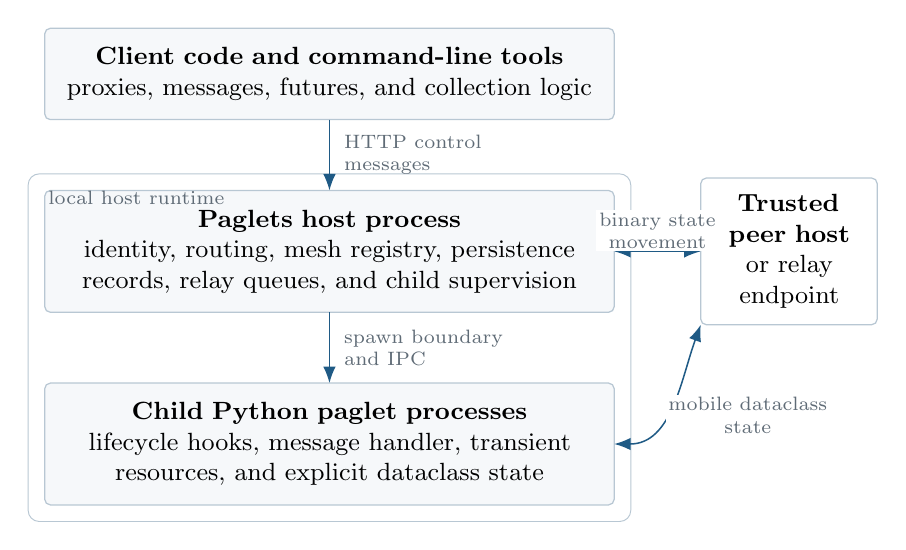
\begin{tikzpicture}[
  node distance=9mm,
  font=\small,
  every node/.style={outer sep=0pt}
]
\node[pagletsLayer] (client)
  {\textbf{Client code and command-line tools}\\
   proxies, messages, futures, and collection logic};
\node[pagletsLayer, below=of client] (host)
  {\textbf{Paglets host process}\\
   identity, routing, mesh registry, persistence records, relay queues, and child supervision};
\node[pagletsLayer, below=of host] (child)
  {\textbf{Child Python paglet processes}\\
   lifecycle hooks, message handler, transient resources, and explicit dataclass state};
\node[pagletsSide, right=11mm of host] (peer)
  {\textbf{Trusted peer host}\\
   or relay endpoint};
\node[draw=pagletsRule, rounded corners=4pt, line width=0.35pt,
      inner xsep=6pt, inner ysep=6pt, fit=(host) (child),
      name=runtime] {};
\node[anchor=north west, font=\scriptsize\color{pagletsMuted}]
  at ([xshift=4pt,yshift=-3pt]runtime.north west) {local host runtime};

\draw[pagletsArrow] (client) -- node[right=2pt, align=left,
  font=\scriptsize\color{pagletsMuted}]
  {HTTP control\\messages} (host);
\draw[pagletsArrow] (host) -- node[right=2pt, align=left,
  font=\scriptsize\color{pagletsMuted}]
  {spawn boundary\\and IPC} (child);
\draw[pagletsMeshArrow] (host.east) -- node[above, align=center,
  fill=white, inner sep=1pt, font=\scriptsize\color{pagletsMuted}]
  {binary state\\movement} (peer.west);
\draw[pagletsMeshArrow] (child.east) to[out=0,in=-110] node[pos=0.42, right,
  align=center, fill=white, inner sep=1pt, font=\scriptsize\color{pagletsMuted}]
  {mobile dataclass\\state} (peer.south west);
\end{tikzpicture}
\caption{Simplified Paglets runtime architecture. The mobile part is the explicit dataclass state plus an importable class reference; active behavior runs in supervised child processes.}
\label{fig:architecture}
\end{figure}

Remote control uses an HTTP API. Small control data is JSON. Movement uses a
binary state envelope rather than forcing large mobile state through JSON. The
runtime streams large payloads for host-to-host movement and uses a local
handoff path when movement stays inside the same host process. The same design
supports the mesh benchmark example, where a traveler paglet moves across host
pairs and records directional movement timing.

Hosts can discover each other through a mesh registry. Mesh entries include
version information so that a paglet is not sent to a host that probably cannot
import the same classes. For networks where inbound ports are difficult, a
relay mode allows outbound-only hosts to communicate through a public HTTPS
endpoint. In shared networks and relay deployments, API-key authentication
should be enabled. This is a practical authentication layer, not a substitute
for a full mobile-code sandbox.

\section{What Paglets Does Differently}

The most important difference from classical Aglets is that Paglets separates
mobile state from installed code. Aglets emerged in a Java setting where mobile
code, object serialization, bytecode portability, and platform security were
central concerns. Paglets assumes a different deployment model: code is shipped
by normal software delivery mechanisms, and mobile execution means moving a
known class reference plus explicit state between hosts that already trust and
understand that code.

This gives Paglets a smaller but sharper contract:

\begin{enumerate}[leftmargin=*]
\item \textbf{State is explicit.} A paglet moves with a dataclass, so authors
  decide what is durable and mobile.
\item \textbf{Code is importable, not uploaded.} Target hosts must have the same
  package or application code available by module path.
\item \textbf{Processes isolate active agents.} Each active paglet runs outside
  the host process, improving crash containment and CPU parallelism.
\item \textbf{Messages stay simple.} The control plane is JSON-oriented, while
  mobile state can use a binary envelope for Python dataclass values.
\item \textbf{Security assumptions are explicit.} Paglets is intended for
  trusted meshes. It does not claim to safely execute arbitrary code from
  unknown senders.
\end{enumerate}

These differences make Paglets less ambitious than strong mobile-code systems,
but more approachable for Python projects where the application owner controls
the participating hosts. The model is especially natural when hosts are
development machines, lab machines, edge devices, compute nodes, or servers in
one administrative domain.

\section{How Paglets Can Be Used}

Paglets is a good fit when moving a compact stateful computation is simpler
than centralizing all data access. Practical examples include:

\paragraph{Infrastructure inspection.}
A paglet can visit hosts, query local disk usage, service status, logs, package
versions, or machine metadata, and return a summarized report. This avoids
streaming raw logs or opening every local interface to a central service.

\paragraph{Data-local analytics.}
When data is large or sensitive, a paglet can move to the data-holding host,
perform filtering or aggregation locally, and return only compact results. This
pattern is useful for local search, privacy-preserving summaries, and
per-site metrics.

\paragraph{Distributed benchmarking and examples.}
The project includes example agents and CLIs for system information, mesh
information, Pi computation, search, performance checks, and mesh movement
benchmarking. These examples exercise the actual runtime paths: paglets are
created, cloned, moved, messaged, and collected rather than mocked as static
function calls.

\paragraph{Stateful workflows.}
A long-running workflow can carry progress, partial results, retry state, an
itinerary, and next-step logic. Instead of requiring a central orchestrator to
drive every small action, the workflow object can continue from the host where
it currently has useful local context.

\paragraph{Agent-to-agent systems.}
Resident service paglets can represent local expertise: disk inspection,
process information, logs, instruments, databases, model adapters, or other
host-bound resources. Visiting paglets communicate with those resident agents
through messages and proxies. This preserves local control while still allowing
mobile coordination.

\paragraph{AI-assisted work contexts.}
For LLM-backed systems, the mobile part often does not need to be the model. It
can be the work context: task description, constraints, memory summary, partial
findings, host itinerary, and tool permissions. A paglet can carry that context
to a host that has a local model adapter or domain service, ask for analysis,
and return with summarized results.

\section{Evaluation}

The following measurements use two hosts connected over a private 1 Gbit/s LAN:
a 2022 Mac Studio with an Apple M1 Max and 32 GB RAM, and a Windows 11 Pro 25H2
workstation with an Intel Core i7-8700K CPU, 64 GB RAM, and an NVIDIA GeForce
GTX 1080 Ti. Both hosts used explicit LAN bindings on port 8765. The movement
benchmark ran ten repeats for each payload size, with seven clock probes per
arrival host. The performance benchmark ran for two seconds per CPU and memory
kernel and used 64 MB temporary disk files. Both hosts reported Python 3.14.6
during the performance run. These measurements are intended to characterize
this Paglets runtime path on one practical mesh; they are not calibrated
hardware or network benchmarks.

\subsection{Movement Across Payload Sizes}

The mesh movement benchmark sent one traveler paglet across every directed host
pair, including self-pairs, for ten repeats. Each run measured 40 movements and
reported no movement errors. Table~\ref{tab:movement-summary} summarizes the
end-to-end movement series. Average movement time stayed below 0.34 s through
16 MB payloads, rose to 0.69 s at 64 MB, and reached 8.76 s at 1 GB. At large
payloads, benchmark time is dominated by end-to-end state movement rather than
clock probes or route overhead.

\begin{table}[H]
\centering
\small
\caption{Mesh movement summary for the dense payload series. Times are seconds.}
\label{tab:movement-summary}
\begin{tabular}{lrrrrrr}
\toprule
Payload & Moves & Avg. move & Travel & Probe round trips & Overhead & Overall \\
\midrule
0 & 40 & 0.219 & 8.766 & 19.688 & 10.922 & 20.400 \\
1 MB & 40 & 0.229 & 9.160 & 20.121 & 10.961 & 20.812 \\
4 MB & 40 & 0.246 & 9.829 & 20.720 & 10.891 & 21.460 \\
16 MB & 40 & 0.334 & 13.377 & 24.327 & 10.950 & 25.083 \\
64 MB & 40 & 0.694 & 27.769 & 38.578 & 10.808 & 39.651 \\
256 MB & 40 & 2.111 & 84.454 & 101.976 & 17.523 & 104.149 \\
512 MB & 40 & 4.112 & 164.479 & 195.749 & 31.271 & 199.492 \\
1 GB & 40 & 8.763 & 350.519 & 410.063 & 59.544 & 417.017 \\
\bottomrule
\end{tabular}
\end{table}

Figure~\ref{fig:mesh-latency} shows directional movement latency by payload
size. Cross-host movement is asymmetric in this run: at 1 GB, Mac-to-Windows
movement averaged 16.98 s, while Windows-to-Mac averaged 12.66 s. Same-host
movement was faster, but also host-dependent: Mac self-movement averaged 1.29 s
at 1 GB, while Windows self-movement averaged 4.12 s. This reflects the
combined runtime, host, OS, storage, and LAN conditions of this specific mesh.

\begin{figure}[H]
\centering
\includegraphics[width=0.92\linewidth]{build/figures/mesh_latency.pdf}
\caption{Mean paglet movement time by payload size and direction. The zero-payload baseline is listed in Table~\ref{tab:movement-summary}; the log-scaled figure shows nonzero payload runs.}
\label{fig:mesh-latency}
\end{figure}

Figure~\ref{fig:mesh-speed} reports effective payload throughput derived from
the same runs. Byte-throughput units use binary scaling, so MB/s means bytes per
second divided by $1024^2$. Mac self-host payload movement was the fastest path
in this run, peaking at 871 MB/s at 512 MB and remaining 792 MB/s at 1 GB.
Windows self-host movement reached 249 MB/s at 1 GB. Cross-host effective
throughput was lower and asymmetric; at 1 GB it was 81 MB/s for
Windows-to-Mac and 60 MB/s for Mac-to-Windows. These rates are end-to-end
Paglets movement rates, not calibrated network line-rate measurements.

\begin{figure}[H]
\centering
\includegraphics[width=0.92\linewidth]{build/figures/mesh_payload_speed.pdf}
\caption{Effective payload transfer speed by payload size. Values come from Paglets' movement benchmark summaries, grouped by self-host and cross-host delivery relation.}
\label{fig:mesh-speed}
\end{figure}

\subsection{Host Performance}

The host performance benchmark cloned workers to both online mesh hosts and
collected local CPU, memory, and disk metrics. Table~\ref{tab:host-performance}
reports the successful single-core and multi-process CPU measurements, memory
copy throughput, and the highest combined read/write disk result for each host.
The ``errors'' column counts benchmark subtests that failed on that host. In
this run, both hosts completed all reported CPU, memory, and disk subtests; no
host-level errors or cleanup errors were reported.

\begin{table}[H]
\centering
\scriptsize
\caption{Host-local performance benchmark results. Byte-throughput columns use binary-scaled GB/s. CPU columns show single-core/multi-process rates.}
\label{tab:host-performance}
\setlength{\tabcolsep}{3.5pt}
\begin{tabular}{llrrrrrrrr}
\toprule
Host & Python & CPUs & Int & Float & SHA & Mem & Disk wr/read & Meta & Errors \\
\midrule
mac-studio & 3.14.6 & 10 & 12.94 / 87.32 & 13.34 / 105.08 & 2.04 / 16.02 & 43.04 & 2.93 / 16.52 & 7,923 & 0 \\
windows11 & 3.14.6 & 12 & 8.25 / 43.25 & 9.97 / 48.32 & 0.50 / 3.01 & 14.44 & 3.79 / 1.74 & 1,746 & 0 \\
\bottomrule
\end{tabular}
\end{table}

\Needspace{0.30\textheight}
\section{Software Availability and Reproducibility}

Paglets is available as an MIT-licensed open-source project on GitHub
\cite{pagletsSoftware}. User documentation is published separately
\cite{pagletsDocs}. The paper source, benchmark JSON files, derived tables, and
plotting scripts are kept under \texttt{papers/paglets-application-note/}; the
paper-specific branch is \texttt{overview-paper}, mirrored from the main
repository history. The manuscript is rebuilt from the repository root with
\texttt{make -C papers/paglets-application-note}, which derives TSV files from
the checked-in benchmark JSON using \texttt{jq}, renders figures with
\texttt{gnuplot}, and runs \texttt{latexmk}. The benchmark hosts reported
Python 3.14.6, and the mesh runs used the project's development mesh version
label, \texttt{dev}.

\section{Limitations and Appropriate Boundaries}

Paglets should not be used as a replacement for ordinary HTTP APIs, queues, or
job runners when a request/response service is simpler. It is also not a secure
execution environment for unknown code. Hosts must already have compatible code
installed, classes must be importable by module path, and movement does not
preserve Python stacks, threads, sockets, or arbitrary live resources.

The process-per-paglet design gives useful isolation, but it means very small
high-frequency work should be batched or implemented as resident service
operations. Message handling is serial per paglet instance, so a parent paglet
should avoid blocking inside a handler while waiting for child result messages
that need the same mailbox. A better pattern is to start work, return quickly,
let workers send result messages, and expose a separate status or summary
message for collection.

The trust boundary should be considered part of the programming model. Paglets
is appropriate for trusted local development, lab networks, controlled servers,
and authenticated relay deployments. It is not designed to receive arbitrary
agents from the public Internet.

\section{Conclusion}

Aglets demonstrated that mobile agents could be programmed as first-class
distributed objects with lifecycle, identity, messaging, and movement. Paglets
revisits that idea for Python by choosing an explicit and intentionally
bounded form of mobility. A paglet moves as durable dataclass state plus a
reference to already-installed behavior. The runtime supplies host management,
process isolation, message passing, persistence, mesh discovery, and transport.

The result is not a universal distributed-computing abstraction. It is a
practical tool for experiments and trusted environments where stateful work
benefits from moving to the machine that has the data, services, devices, or
local context. In that narrower domain, Paglets keeps the attractive parts of
the Aglets model while replacing implicit mobile-code assumptions with a
Python-friendly operational contract.

\bibliographystyle{plainurl}
\bibliography{references}

\end{document}
